\documentclass[tikz]{standalone}
\usetikzlibrary{arrows,shapes,positioning,shadows,trees}
\usetikzlibrary{mindmap}


%\tikzset{
%  basic/.style  = {draw, text width=2cm, drop shadow, font=\sffamily, rectangle},
%  root/.style   = {basic, rounded corners=2pt, thin, align=center,
%                   fill=green!80},
%  interface/.style   = {basic, rounded corners=2pt, thin, align=center,
%                   fill=yellow!30},
%  abstractclass/.style   = {basic, rounded corners=2pt, thin, align=center,
%                   fill=red!30},
%  class/.style   = {basic, rounded corners=2pt, thin, align=center,
%                   fill=green!30},
%  level 2/.style = {basic, rounded corners=6pt, thin,align=center, fill=green!60,
%                   text width=8em},
%  level 3/.style = {basic, thin, align=left, fill=pink!60, text width=6.5em}
%}


\tikzset{
	property/.style = {concept, inner sep = 0, concept color = green!80!black},
	class/.style = {concept, concept color = green!50!blue},
	abstract class/.style = {concept, concept color = green!30!blue},
	interface/.style = {concept, concept color = blue!90!black},
	comment/.style  = {
		label = {
			[text = red, 
			inner sep = 0,
			rectangle, 
			font=\tiny, 
			above = -0.45]
			above:#1}},
	add/.style 		= { comment = {Add}},
	other/.style 	= {comment = {Other}},
}

\begin{document}
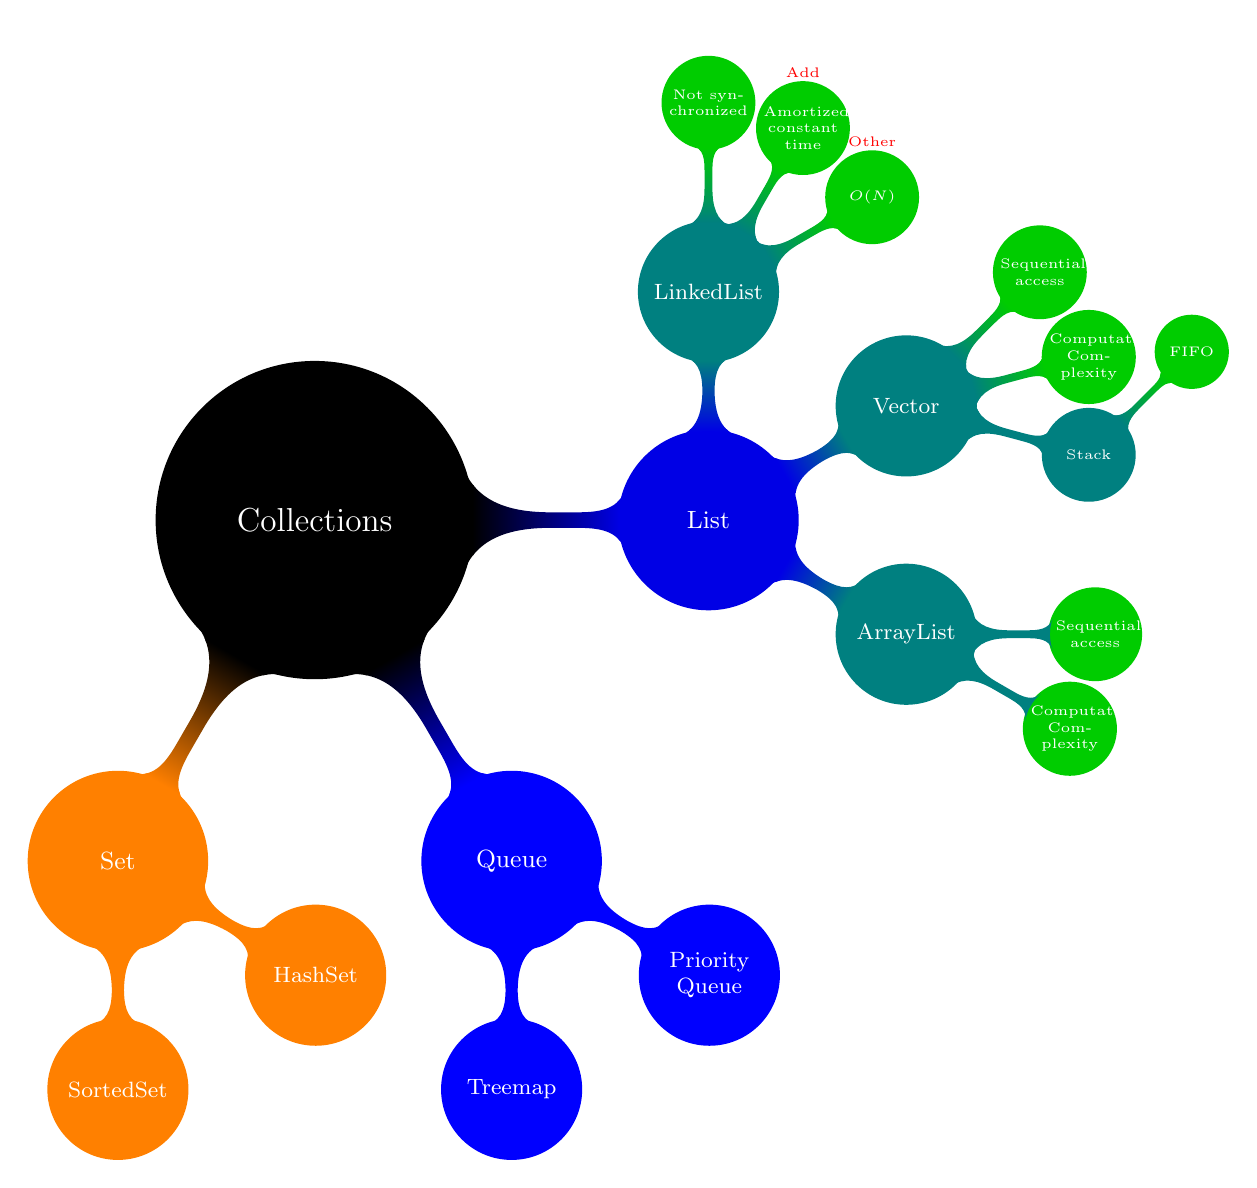
\begin{tikzpicture}
\path[mindmap,concept color=black,text=white]
	node[concept] {Collections}[clockwise from=0]
% note that ?sibling angle? can only be defined in % ?level 1 concept/.append style={}?
		child[interface] {
			node[concept] {List}
			[clockwise from=90]
			child[class] { 
				node[concept] {LinkedList} 
				child[property] { node[concept] {Not synchronized}}
				child[property] { node[concept, add] {
					Amortized constant time}}
				child[property] { node[concept, other] {
					$O(N)$}}
				}
			child[class] { 
				node[concept] {Vector} 
				[clockwise from=45]
				child[property] { node[concept] {Sequential access}}
				child[property] { node[concept] {Computational Complexity}}
				child[class] { 
					node[class] {Stack}
					child[property]{ node[concept] {FIFO}}
					}
				}
			child[class] { 
				node[concept] {ArrayList} 
				[clockwise from=0]
				child { node[property] {Sequential access}}
				child { node[property] {Computational Complexity}}
				}
		}
		child[concept color=blue] {
			node[concept] {Queue}
			[clockwise from=-30]
			child { node[concept] {Priority Queue} } 
			child { node[concept] {Treemap} }
		}
		child[concept color=orange] {
			node[concept] {Set}
			[clockwise from=-30]
			child { node[concept] {HashSet} } 
			child { node[concept] {SortedSet} }
		}
%		child[concept color=red] { 
%			node[concept] {technical} 
%		} 
%		child[concept color=orange] { 
%			node[concept] {theoretical} 
%		}
		;
\end{tikzpicture}
\end{document}